\documentclass[12pt]{article}
\usepackage[a4paper, total={6in, 8in}]{geometry}
\usepackage{polski}
\usepackage{adjustbox}
\usepackage{pgfplots}
\usepackage{amsmath}
\usepackage{multirow}

\setlength{\parindent}{0pt}
\setlength{\oddsidemargin}{-15pt}
\setlength{\textwidth}{480pt}
\setlength{\textheight}{730pt}

\newcommand{\dpartial}[2]{\frac{\partial #1}{\partial #2}}
\newcommand{\physdpartial}[2]{\left( \dpartial{#1}{#2} \right)^2}
\newcommand{\powfrac}[2]{\left( \frac{#1}{#2} \right)^2}
\newcommand{\powsq}[1]{\left( #1 \right)^{\frac{3}{2}}}

\author{Michał Puchyr, Dawid Chudzicki}
\title{Sprawozdanie z ćw 53 -- PRAWO OHMA DLA PRĄDU PRZEMIENNEGO}

\pgfplotsset{scaled x ticks=false}

\begin{document}
\maketitle

\section{Cel ćwiczenia}
\begin{itemize}
    \item Wyznaczenie wartości indukcyjności cewki i pojemności kondensatora przy zastosowaniu prawa
    Ohma dla prądu przemiennego,
    \item Sprawdzenie prawa Ohma dla prądu przemiennego dla
    szeregowego układu złożonego z opornika, cewki indukcyjnej i kondensatora.
\end{itemize}

\section{Wstęp teoretyczny}

\textbf{Prąd przemienny} (AC) -- charakterystyczny przypadek prądu elektrycznego okresowo zmiennego, 
w którym wartości chwilowe podlegają zmianom w powtarzalny, okresowy sposób, z określoną częstotliwością. 
Wartości chwilowe natężenia prądu przemiennego przyjmują naprzemiennie wartości dodatnie i ujemne. 

Największe znaczenie praktyczne mają prąd i napięcie o przebiegu sinusoidalnym. W żargonie technicznym nazwa prąd przemienny często oznacza po prostu \textbf{prąd sinusoidalny}. \bigskip

\textbf{Kondensator} -- element elektroniczny bierny zbudowany z dwóch przewodników -- inaczej okładek lub elektrod -- 
rozdzielonych dielektrykiem; przechowuje on energię w postaci pola elektrycznego.

Pojemność kondensatora mierzy zdolność kondensatora do magazynowania ładunku elektrycznego.

Jednostką pojemności jest farad (F). 

Kondensatory są wykorzystywane w elektronice do różnych celów, na przykład do filtrowania sygnałów, 
magazynowania energii, stabilizacji napięcia, generowania sygnałów i wielu innych zastosowań. \bigskip

\textbf{Cewka indukcyjna} to element elektryczny składający się z przewijanej spirali z drutu lub taśmy ferromagnetycznej, 
który wykorzystuje zjawisko elektromagnetycznej indukcji do magazynowania energii w postaci pola magnetycznego. 

Indukcyjność jest podstawowym parametrem elektrycznym opisującym cewkę.
Prąd płynący w obwodzie wytwarza skojarzony z nim strumień magnetyczny.

Jednostką indukcyjności jest henr [H].


Indukcyjność definiuje się jako stosunek tego strumienia i prądu, który go wytworzył:

$$ L = k \frac{\Phi}{i} $$
Współczynnik $k$ zależy od geometrii układu, a więc między innymi od kształtu cewki, liczby zwojów, grubości użytego drutu. Indukcyjność cewki zależy również od przenikalności magnetycznej rdzenia.

\bigskip
Wykaz przyrządów :
\begin{itemize}
    \item Generator AG 1012F
    \item Woltomierz napięcia przemiennego
    \item Miliamperomierz prądu przemiennego
    \item Zestaw składający się z oporników, cewek indukcyjnych i kondensatorów
\end{itemize}

Oporność badanego opornika : $ R = (157 \pm 3) \Omega $

Oporność cewki indukcyjnej : $ R_{L2} = (0,60 \pm 0,05) \Omega $

Przedział częstotliwości pomiarowej dla pojemności $C_3$ : od 50 Hz do 200Hz

\section{Przykładowe obliczenia}
\subsection{Niepewności mierników}

Niepewność woltomierza

Dla zakresu:
\begin{itemize}
    \item 4V : $ \pm 0,8 \% \ \textrm{rdg} + 3\textrm{dgt}$ \quad dgt $=1$mV
    \item 40V : $ \pm 2.5 \% \ \textrm{rdg} + 5\textrm{dgt} $ \quad dgt $=10$mV
\end{itemize} \bigskip

Np.
$$ u_b(U) = \frac{0,008 \cdot 1,016 + 3 \cdot 0,001}{\sqrt{3}} = 0,00642 \approx 0,0065[V] $$ \bigskip

Niepewność amperomierza (dla prądu zmiennego)

Dla zakresu:
\begin{itemize}
    \item 40 mA : $ \pm 1.5\% \ \textrm{rdg} + 3\textrm{dgt} $ \quad dgt $=10\mu$A
    \item 400 mA : $ \pm 1.5\% \ \textrm{rdg} + 3\textrm{dgt} $ \quad dgt $=100\mu$A
\end{itemize}

Np. 
$$ u_b(I) = \frac{0,015 \cdot 2,090 + 3 \cdot 0,00001}{\sqrt3} = 0,01811 \approx 0,019[mA]$$\bigskip

Niepewność ustalenia częstotliwości generatora:
\begin{itemize}
    \item $ \pm 1\% \ \textrm{rdg} \pm 1 \textrm{Hz} $
\end{itemize}

Np.
$$ u_b(f) = \frac{0,01 \cdot 125 + 1}{\sqrt{3}} = 1.29903 \approx 1,3[Hz] $$ 

\subsection{Wyznaczenie pojemności kondesatora}

Obliczenie pojemności kondensatora:
$$ C = \frac{1}{2 \pi f \sqrt{Z_C^2 - R^2}} = \frac{1}{2 \pi \cdot 125 \sqrt{470^2 - 157^2}} = 2,874115253^{-6} \approx 2,874116^{-6}[F] $$

Wyznaczenie niepewności złożonej pojemności kondensatora:

$$ u_c(C) = \sqrt{ \physdpartial{C}{f} \cdot u(f)^2 + \physdpartial{C}{Z_C} \cdot u(Z_C)^2 + \physdpartial{C}{R} \cdot u(R)^2 } $$
$$ = \sqrt{ \powfrac{-1}{2 \pi f^2 \sqrt{Z_C^2 - R^2}} \cdot u(f)^2 + \powfrac{-Z_C}{2 \pi f \powsq{Z_c^2 - R^2} } \cdot u(Z_C)^2 + \powfrac{R}{2 \pi f \powsq{Z_C^2 - R^2}} \cdot u(R)^2 } $$
$$ = \sqrt{ \powfrac{-1}{2 \pi \cdot 125^2 \sqrt{470^2 - 157^2}} \cdot 1,3^2 + \powfrac{-470}{2 \pi \cdot 125 \powsq{470^2 - 157^2} } \cdot 2^2 + \powfrac{157}{2\pi \cdot 125 \powsq{470^2 - 157^2} } \cdot 3^2 } $$
$$ = 3,3624^{-8}[F] $$

\subsection{Wyznaczenie indukcyjności cewki}

Obliczenie indukcyjności cewki:

$$ L = \frac{ \sqrt{Z_L^2 - (R + R_L)^2} }{2 \pi f} = \frac{ \sqrt{ 164,64^2 - (157 + 0,60)^2 }}{2 \pi \cdot 125} = 0,060644 \approx 0,061[H] $$

Wyznaczenie niepewności złożonej indukcyjności cewki

$$ u_c(L) = \sqrt{ \physdpartial{L}{Z_L} \cdot u(Z_L)^2 + \physdpartial{L}{R} \cdot u(R)^2 + \physdpartial{L}{R_L} \cdot u(R_L)^2 + \physdpartial{L}{f} \cdot u(f)^2 } $$

$$ = u_c(L) = \sqrt{ \powfrac{Z_L}{2\pi f \sqrt{Z_L^2 - (R + R_L)^2}} \cdot u(Z_L)^2 + \powfrac{-(R + R_L)}{2\pi f \sqrt{Z_L^2 - (R + R_L)^2}} \cdot u(R)^2 } $$
$$ \overline{+ \powfrac{-(R + R_L)}{2\pi f \sqrt{Z_L^2 - (R + R_L)^2}} \cdot u(R_L)^2 + \powfrac{- \sqrt{Z_L^2 - (R - R_L)^2}}{2 \pi f^2} \cdot u(f)^2 } $$
$$ = 0,0131514 \approx 0,014[H]$$

\pagebreak

\subsection{Sprawdzenie słuszności prawa Ohma dla prądu przemiennego}

Wyznaczenie zawady nr 2 dla układu szeregowego RLC:

$$ Z_2 = \sqrt{(R + R_L)^2 + \left(2 \pi f L - \frac{1}{2 \pi f C}\right)^2} = 425,625862 $$

Wyznaczenie niepewności złożonej dla zawady nr 2:

$$ u(Z_2) = \sqrt{ \powfrac{R + R_L}{\sqrt{(R + R_L)^2 + \left(2 \pi f L - \frac{1}{2\pi f C}\right)^2}} \cdot u(R)^2 + \powfrac{R+R_L}{\sqrt{(R + R_L)^2 + \left(2 \pi f L - \frac{1}{2\pi f C}\right)^2}} \cdot u(R_L)^2 } $$
$$ \overline{ \powfrac{\left( 2\pi f L - \frac{1}{2 \pi f C} \right) \cdot 2 \pi f}{\sqrt{(R + R_L)^2 + \left(2 \pi f L - \frac{1}{2\pi f C}\right)^2}} \cdot u(L)^2 + 
\powfrac{\left(2 \pi f L - \frac{1}{2 \pi f C}\right) \cdot \left( 2\pi L + \frac{1}{2 \pi f^2 C} \right)}{\sqrt{(R + R_L)^2 + \left(2 \pi f L - \frac{1}{2\pi f C}\right)^2}} \cdot u(f)^2} $$
$$ \overline{ \powfrac{\left( 2 \pi f L - \frac{1}{2 \pi f C} \right) \cdot \frac{1}{2 \pi C^2 f}}{\sqrt{(R + R_L)^2 + \left(2 \pi f L - \frac{1}{2\pi f C}\right)^2}} \cdot u(C)^2 } 
= 11,7873 $$

\pagebreak

\section{Pomiary i opracowanie wyników}

\subsection{Wyznaczanie pojemności kondensatora (RC)}

\begin{center}
\begin{tikzpicture}
    \begin{axis}[
        xlabel={$I[A]$},
        ylabel={$U[V]$},
        xmin=0,
        xmax=0.025,
        ymin=0,
        ymax=12,
        xtick={0,0.005,0.01,0.015,0.02,0.025},
        ytick={0,2,4,6,8,10,12},
        grid=major,
        grid style={dashed,gray!50},
        width=14cm,
        height=10cm,
        axis lines=middle,
        enlargelimits=0.05,
        tick align=outside,
        legend style={at={(0.5,-0.15)},anchor=north},
        legend cell align=left,
        mark size=2.5pt,
        xticklabel style={
            /pgf/number format/fixed,
            /pgf/number format/precision=5
        },
    ]
    \addplot[red, domain=0:0.025, dashed] {469.49*x}; \addlegendentry{Regresja liniowa: $y = 469,49x$}
    \addplot[blue, only marks] coordinates {
        (0.00209,1.016)
        (0.00413,2.03)
        (0.00642,3.046)
        (0.0086,4.10)
        (0.0109,5.12)
        (0.01311,6.15)
        (0.01487,7.17)
        (0.01748,8.16)
        (0.01975,9.18)
        (0.02175,10.15)
    };
    \end{axis}
    \end{tikzpicture}

    \textbf{Wykres zależności napięcia od natężenia}
\end{center}

\begin{table}[h]
    \centering
    \caption{Wyniki pomiarów i obliczeń}
    \label{tab:tabela1}
    \begin{tabular}{|c|c|c|c|c|c|c|c|c|c|c|} \hline
    Lp & U[V] & u(U)[V] & I[mA] & u(I)[mA] & Z\textsubscript{c} & u(Z\textsubscript{c}) & $f$[Hz] & u($f$)[Hz] & C[F] & u(C)[F] \\ \hline
    1 & 1,0160 & 0,0065 & 2,090 & 0,019 & \multirow{10}{*}{470} & \multirow{10}{*}{2} & \multirow{10}{*}{125,0} & \multirow{10}{*}{1,3} & \multirow{10}{*}{2,874116$^{-6}$} & \multirow{10}{*}{3,3624$^{-8}$} \\ \cline{1-5}
    2 & 2,034 & 0,012 & 4,130 & 0,036 & & & & & & \\ \cline{1-5}
    3 & 3,046 & 0,016 & 6,420 & 0,056 & & & & & & \\ \cline{1-5}
    4 & 4,100 & 0,089 & 8,600 & 0,075 & & & & & & \\ \cline{1-5}
    5 & 5,12 & 0,11 & 10,900 & 0,095 & & & & & & \\ \cline{1-5}
    6 & 6,15 & 0,12 & 13,11 & 0,12 & & & & & & \\ \cline{1-5}
    7 & 7,17 & 0,14 & 14,87 & 0,13 & & & & & & \\ \cline{1-5}
    8 & 8,16 & 0,15 & 17,48 & 0,16 & & & & & & \\ \cline{1-5}
    9 & 9,18 & 0,17 & 19,75 & 0,18 & & & & & & \\ \cline{1-5}
    10 & 10,15 & 0,18 & 21,75 & 0,19 & & & & & & \\ \hline
    \end{tabular}
\end{table}

\subsection{Wyznaczenie indukcyjności cewki}

\begin{center}
    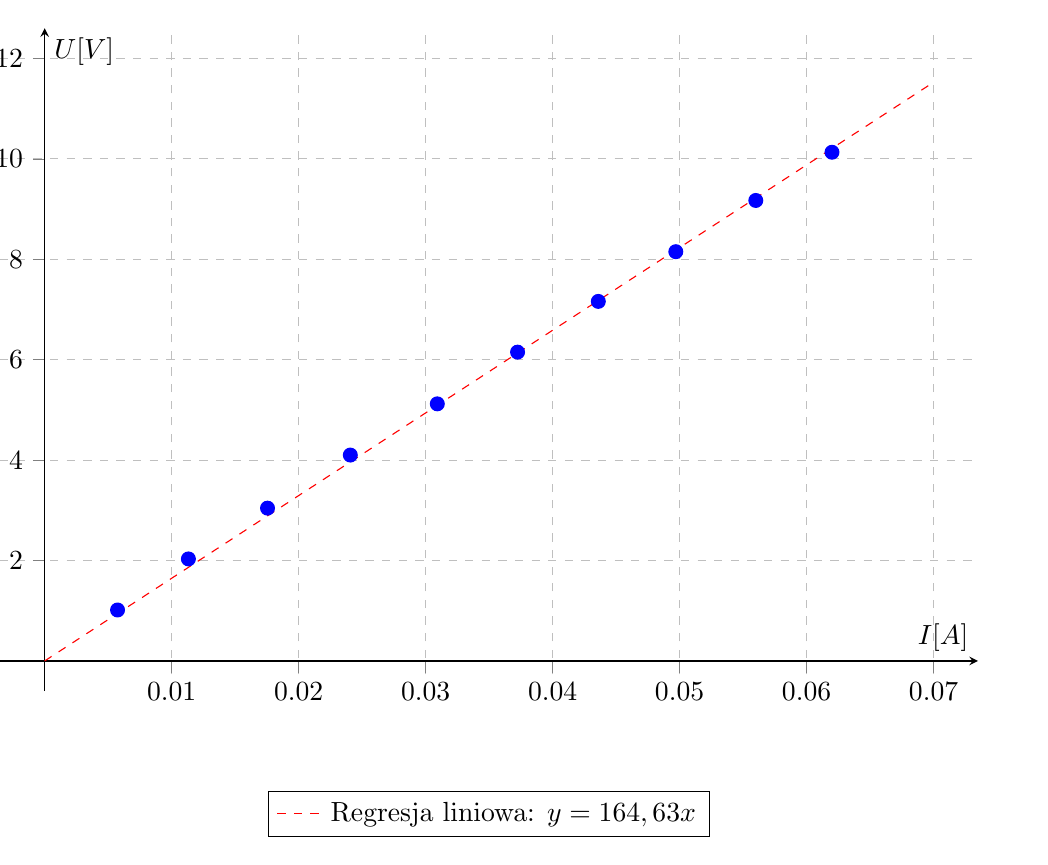
\begin{tikzpicture}
        \begin{axis}[
            xlabel={$I[A]$},
            ylabel={$U[V]$},
            xmin=0,
            xmax=0.07,
            ymin=0,
            ymax=12,
            xtick={0,0.01,0.02,0.03,0.04,0.05, 0.06, 0.07},
            ytick={0,2,4,6,8,10,12},
            grid=major,
            grid style={dashed,gray!50},
            width=14cm,
            height=10cm,
            axis lines=middle,
            enlargelimits=0.05,
            tick align=outside,
            legend style={at={(0.5,-0.15)},anchor=north},
            legend cell align=left,
            mark size=2.5pt,
            xticklabel style={
                /pgf/number format/fixed,
                /pgf/number format/precision=5
            },
        ]
        \addplot[red, domain=0:0.07, dashed] {164.63*x}; \addlegendentry{Regresja liniowa: $y = 164,63x$}
        \addplot[blue, only marks] coordinates {
            (0.00574, 1.0150) (0.01132, 2.032) (0.01755, 3.043) (0.02407, 4.100) (0.03092, 5.12) (0.03724, 6.150) (0.0436, 7.16) (0.0497, 8.15) (0.056, 9.17) (0.062, 10.13)
        };
        \end{axis}
        \end{tikzpicture}
    
        \textbf{Wykres zależności napięcia od natężenia}
\end{center}

\begin{table}[h]
    \centering
    \caption{Wyniki pomiarów i obliczeń dla wyznaczenia indukcyjności cewki}
    \label{tab:Wyniki pomiarów i obliczeń}
    \begin{tabular}{|c|c|c|c|c|c|c|c|c|c|c|} \hline
    Lp & U[V] & u(U)[V] & I[mA] & u(I)[mA] & Z\textsubscript{L} & U(Z\textsubscript{L}) & $f$[Hz] & u($f$)[Hz] & L[H] & u(L)[Hz] \\ \hline
    1 & 1,0150 & 0,0065 & 5,74 & 0,05 & \multirow{10}{*}{164,64} & \multirow{10}{*}{0,81} & \multirow{10}{*}{125,0} & \multirow{10}{*}{1,3} & \multirow{10}{*}{0,061} & \multirow{10}{*}{0,014} \\ \cline{1-5}
    2 & 2,032 & 0,012 & 11,320 & 0,099 & ~ & ~ & ~ & ~ & ~ & ~ \\ \cline{1-5}
    3 & 3,043 & 0,016 & 17,55 & 0,16 & ~ & ~ & ~ & ~ & ~ & ~ \\ \cline{1-5}
    4 & 4,100 & 0,089 & 24,07 & 0,21 & ~ & ~ & ~ & ~ & ~ & ~ \\ \cline{1-5}
    5 & 5,12 & 0,11 & 30,92 & 0,27 & ~ & ~ & ~ & ~ & ~ & ~ \\ \cline{1-5}
    6 & 6,15 & 0,12 & 37,24 & 0,33 & ~ & ~ & ~ & ~ & ~ & ~ \\ \cline{1-5}
    7 & 7,16 & 0,14 & 43,6 & 0,38 & ~ & ~ & ~ & ~ & ~ & ~ \\ \cline{1-5}
    8 & 8,15 & 0,15 & 49,7 & 0,44 & ~ & ~ & ~ & ~ & ~ & ~ \\ \cline{1-5}
    9 & 9,17 & 0,17 & 56 & 0,49 & ~ & ~ & ~ & ~ & ~ & ~ \\ \cline{1-5}
    10 & 10,13 & 0,18 & 62 & 0,54 & ~ & ~ & ~ & ~ & ~ & ~ \\ \hline
    \end{tabular}
\end{table}

\subsection{Sprawdzenie słuszności prawa Ohma dla prądu przemiennego}

\begin{center}
    \begin{tikzpicture}
        \begin{axis}[
            xlabel={$I[A]$},
            ylabel={$U[V]$},
            xmin=0,
            xmax=0.025,
            ymin=0,
            ymax=10,
            xtick={0,0.005,0.010,0.015,0.020,0.025},
            ytick={0,2,4,6,8,10,12},
            grid=major,
            grid style={dashed,gray!50},
            width=14cm,
            height=10cm,
            axis lines=middle,
            enlargelimits=0.05,
            tick align=outside,
            legend style={at={(0.5,-0.15)},anchor=north},
            legend cell align=left,
            mark size=2.5pt,
            xticklabel style={
                /pgf/number format/fixed,
                /pgf/number format/precision=5
            },
        ]
        \addplot[red, domain=0:0.07, dashed] {464.16*x}; \addlegendentry{Regresja liniowa: $y = 464,16x$}
        \addplot[blue, only marks] coordinates {
            (0.00218, 1.015) (0.00439, 2.034) (0.0066, 3.046) (0.00881, 4.11) (0.01102, 5.13) (0.01323, 6.15) (0.01544, 7.17) (0.01759, 8.16) (0.01981, 9.18) (0.02187, 10.15)
        };
        \end{axis}
        \end{tikzpicture}
    
        \textbf{Wykres zależności napięcia od natężenia}
\end{center}

\begin{table}[h]
    \centering
    \caption{Wyniki pomiarów i obliczeń dla wyznaczenia zawady układu}
    \begin{tabular}{|c|c|c|c|c|c|c|c|c|c|c|}
    \hline
    Lp & U[V] & u(U)[V] & I[mA] & u(I)[mA] & Z\textsubscript{1}[$\Omega$] & u(Z\textsubscript{1})[$\Omega$] & $f$[Hz] & u($f$)[Hz] & Z\textsubscript{2}[$\Omega$] & u(Z\textsubscript{2})[$\Omega$] \\ \hline
    1 & 1,015 & 0,0065 & 2,18 & 0,019 & \multirow{10}{*}{464,16} & \multirow{10}{*}{0,29} & \multirow{10}{*}{125,0} & \multirow{10}{*}{1,3} & \multirow{10}{*}{425,6258} & \multirow{10}{*}{11,7873} \\ \cline{1-5}
    2 & 2,034 & 0,012 & 4,39 & 0,039 & ~ & ~ & ~ & ~ & ~ & ~ \\ \cline{1-5}
    3 & 3,046 & 0,016 & 6,6 & 0,058 & ~ & ~ & ~ & ~ & ~ & ~ \\ \cline{1-5}
    4 & 4,11 & 0,089 & 8,81 & 0,077 & ~ & ~ & ~ & ~ & ~ & ~ \\ \cline{1-5}
    5 & 5,13 & 0,11 & 11,02 & 0,096 & ~ & ~ & ~ & ~ & ~ & ~ \\ \cline{1-5}
    6 & 6,15 & 0,12 & 13,23 & 0,12 & ~ & ~ & ~ & ~ & ~ & ~ \\ \cline{1-5}
    7 & 7,17 & 0,14 & 15,44 & 0,14 & ~ & ~ & ~ & ~ & ~ & ~ \\ \cline{1-5}
    8 & 8,16 & 0,15 & 17,59 & 0,16 & ~ & ~ & ~ & ~ & ~ & ~ \\ \cline{1-5}
    9 & 9,18 & 0,17 & 19,81 & 0,18 & ~ & ~ & ~ & ~ & ~ & ~ \\ \cline{1-5}
    10 & 10,15 & 0,18 & 21,87 & 0,19 & ~ & ~ & ~ & ~ & ~ & ~ \\ \hline
    \end{tabular}
\end{table}

\section{Wnioski}

W eksperymencie udało się wyznaczyć pojemność kondensatora, która wynosi około $2,874116^{6} \pm 3,3624^{-8}$F oraz indukcyjność cewki,
która wynosi około $ 0,061 \pm 0,014 $H.

Zostało też udowodnione spełnianie prawa Ohma dla układu z prądem przemiennym. Wskazuje na to zależność liniowa pomiarów napięcia od natężenia.

\end{document}